\documentclass{scrartcl}

% -----------------------------------------------------------
% Pakete

% Layout
\usepackage[utf8]{inputenc}
\usepackage[headsepline]{scrlayer-scrpage}

% Sprachen
\usepackage[ngerman]{babel}

% Formeln & co.
\usepackage{mathtools}
\usepackage{amsmath}
\usepackage{float}
\usepackage{amsthm}
\usepackage{amssymb}
\usepackage{stmaryrd}
\usepackage{physics}
\usepackage{siunitx}
\usepackage[mathscr]{euscript}
\usepackage[shortlabels]{enumitem}

% Malen nach Zahlen
\usepackage{tcolorbox}
\usepackage{tikz}
\usepackage{pgfplots}

% Weitere wichtige Helfer
\usepackage{amsthm}
\usepackage{thmtools}
\usepackage{xifthen}
\usepackage{hyperref}
\usepackage{xspace}

% -----------------------------------------------------------
% Design
\tcbset{sharp corners=all,boxrule=0mm}

% -----------------------------------------------------------
% Umgebungen
\let\oldproof\proof
\let\endoldproof\endproof
\let\proof\relax
\let\endproof\relax
\newenvironment{proof}{\begin{tcolorbox}\begin{oldproof}}{\end{oldproof}\end{tcolorbox}}

% -----------------------------------------------------------
% Toms Divacode
    \usepackage{calrsfs}
\usepackage{thmtools}
\usepackage[usenames,dvipsnames]{xcolor}
\declaretheoremstyle[
    			headfont=\bfseries\sffamily\color{black!70!black}, bodyfont=\normalfont,
    			mdframed={
       				linewidth=1pt,
        			rightline=false, topline=false, bottomline=false,
    			}
			]{Begruendungsbox}
\declaretheoremstyle[
    			headfont=\bfseries\sffamily\color{black!70!black}, bodyfont=\normalfont,
    			mdframed={
       				linewidth=1pt,
        			rightline=false, topline=false, bottomline=false,
    			}
			]{Erinnerungsbox}
\declaretheoremstyle[
    			headfont=\bfseries\sffamily\color{black!70!black}, bodyfont=\normalfont, numbered=no,
    			mdframed={
       				linewidth=false,
        			rightline=false, topline=false, bottomline=false,
    			}
			]{Zusammenfassungsbox}
\declaretheoremstyle[
    			headfont=\bfseries\sffamily\color{black!70!black}, bodyfont=\normalfont, numbered=no,
    			mdframed={
       				linewidth=0.5pt,
        			rightline=0.5pt, topline=false, bottomline=false,
    			}
			]{Voraussetzungsbox}
\declaretheorem[style=Voraussetzungsbox, name=Voraussetzung]{vrr}
\declaretheorem[style=Zusammenfassungsbox, name=Zusammenfassen]{zsmfs}
\newenvironment{Voraussetzung}{\begin{vrr}}{\end{vrr}}
\newenvironment{Zusammenfassen}{\begin{zsmfs}}{\end{zsmfs}}
\declaretheorem[style=Erinnerungsbox, name=Vermutung]{verm}
\declaretheorem[style=Begruendungsbox, name=Begründung]{begr}
\newenvironment{begruendung}{\begin{begr}}{\end{begr}}

\newcommand{\nbra}[1]{\left(#1\right)}
\newcommand{\nsqbra}[1]{\left[#1\right]}
\newcommand{\nset}[1]{\left\{{#1}\right\}}
\newcommand{\lfdef}[2]{\begin{pmatrix}{#1}\\{#2}\end{pmatrix}}
\newcommand{\fdef}[2]{\nbra{#1}_{#2}}
\newcommand{\dabs}[2]{\abs{\abs{#1}}_{#2}}
\newcommand{\Abb}[2]{\text{Abb}\nbra{#1,#2}}
\newcommand{\postref}[1]{\nsqbra{\rightarrow{#1}}}
\newcommand{\anm}[1]{[\textit{#1}]}

\declaretheorem[style=Erinnerungsbox, name=Erinnerung]{Erinnerungsdef}
\newenvironment{Erinnerung}{\begin{Erinnerungsdef}}{\end{Erinnerungsdef}}

\renewcommand{\vec}[1]{\mathbf{#1}}

\newcommand{\diff}[4]{%
			\ifthenelse{\isempty{#2}}
				{\ifthenelse{\isempty{#3}}
					{\ifthenelse{\isempty{#4}}
						{\ensuremath{d#1}}
						{\ensuremath{d^{#4}#1}}}
					{\ifthenelse{\isempty{#4}}
						{\ensuremath{d#1\nbra{#3}}}
						{\ensuremath{d^{#4}#1\nbra{#3}}}}}
				{\ifthenelse{\isempty{#3}}
					{\ifthenelse{\isempty{#4}}
						{\ensuremath{d#1()\nbra{#2}}}
						{\ensuremath{d^{#4}#1()\nbra{#2}}}}
					{\ifthenelse{\isempty{#4}}
						{\ensuremath{d#1\nbra{#3}\nbra{#2}}}
						{\ensuremath{d^{#4}#1\nbra{#3}\nbra{#2}}}}}%
		}
\newcommand{\Diff}[4]{%
			\ifthenelse{\isempty{#3}}
				{\ifthenelse{\isempty{#4}}
					{\ensuremath{\text{D}_{#2}#1}}
					{\ensuremath{\text{D}_{#2}^{#4}#1}}}
				{\ifthenelse{\isempty{#4}}
					{\ensuremath{\text{D}_{#2}#1\nbra{#3}}}
					{\ensuremath{\text{D}_{#2}^{#4}#1\nbra{#3}}}}%
		}
\newcommand{\pdiff}[4]{%
			\ifthenelse{\isempty{#3}}
				{\ifthenelse{\isempty{#4}}
					{\ensuremath{\partial_{#2}#1}}
					{\ensuremath{\partial_{#2}^{#4}#1}}}
				{\ifthenelse{\isempty{#4}}
					{\ensuremath{\partial_{#2}#1\nbra{#3}}}
					{\ensuremath{\partial_{#2}^{#4}#1\nbra{#3}}}}%
		}
\newcommand{\scpr}[2]{\left\langle #1,#2\right\rangle}
\DeclareMathOperator{\mal}{mal}
\DeclareMathOperator{\plus}{plus}
\renewcommand{\neg}{\text{neg}}
\DeclareMathOperator{\inv}{inv}

\newcommand\numberthis{\addtocounter{equation}{1}\tag{\theequation}}
\newenvironment{beh}{\noindent\textbf{\textit{Behauptung.}}}{}
\DeclareMathOperator{\laplace}{\text{lap}}
\newcommand{\Null}[1]{0_{#1}}

\newcommand{\gint}[1]{\int_{[#1]}}
\newcommand{\dint}[2][]{%
				\ifthenelse{\isempty{#2}}{\,d#2}{\,d_{#1}#2}
				}%
\newcommand{\Ell}{\mathcal L}
\newcommand{\Real}[1]{\text{Re}\nbra{#1}}
\newcommand{\Imag}[1]{\text{Im}\nbra{#1}}

\newcommand{\Mengeninklusion}[2]{
	\begin{itemize}
		\item[\enquote{$\subseteq$}] #1
		\item[\enquote{$\supseteq$}] #2
	\end{itemize}}
 \newcommand{\sAlgebra}[1]{{\sigma}\Mengenschriftdesign{Algebra}\nbra{#1}}

\usepackage{xargs}
\newcounter{ex}
			\newcounter{subex}[ex]
			\newcounter{subsubex}[subex]
			
			\setcounter{ex}{1}
 \newcommandx{\aufgabe}[1][1={}]{\ifnumgreater{\theex}{1}{\newpage}{}
				\ifthenelse{\isempty{#1}}	
					{\section*{Aufgabe \theex}\label{ex:\theex}\stepcounter{ex}}
					{\section*{Aufgabe #1}\label{ex:#1}}}
\newcommandx{\subaufgabe}[1][1={}]{\ifthenelse{\isempty{#1}}
					{\stepcounter{subex}\subsection*{(\alph{subex})}\label{subex:\theex-\thesubex}}
					{\stepcounter{subex}\subsection*{(#1)}\label{subex:\theex-#1}}}


% -----------------------------------------------------------
% Blattspezifische Commands


% -------------------------------------------------------
% Allgemein nicht wegzudenken

\let\oldemptyset\emptyset
\let\emptyset\varnothing

\newcommand{\R}{\mathbb{R}}
\newcommand{\N}{\mathbb{N}}
\newcommand{\Z}{\mathbb{Z}}
\newcommand{\Q}{\mathbb{Q}}
\newcommand{\C}{\mathbb{C}}
\newcommand{\Prim}{\mathbb{P}}
\newcommand{\K}{\mathbb K}
\newcommand{\F}{\mathbb{F}}
		
\DeclareMathOperator{\cmath}{\overset\circ\imath}
\DeclareMathOperator\Def{Def}
\DeclareMathOperator\Bild{Bild}

% -------------------------------------------------------
% Kopfzeile

\ihead{Tom Folgmann\\David Jannack}
\chead{Michael Hein\\Blatt 1} % <- hier Blattnummer ergänzen (THEORIE)

\begin{document}

\centerline{\Large\textbf{Computerphysik}}
\noindent\makebox[\linewidth]{\rule{11cm}{1pt}}

\aufgabe
    \subaufgabe
        \begin{itemize}
            \item Microsoft Windows
            \item macOS
            \item Android
            \item iOS
            \item OnePlus OS
            \item MyCloud OS
            \item Playstation, XBOX, Nintendo OSe..
            \item Arch Linux
            \item Ubuntu
            \item Debian
            \item Asahi Project/Linux
            \item Raspberry Pi OS
        \end{itemize}
        Es gibt mobile und stationäre (Desktop) Betriebssysteme, sowie speziellere für einzelne Anwendungsbereiche (MyCloud OS). Desweiteren kann man zwischen (teilweise) open-source (Arch Linux, Asahi Projec) und kommerziellen (macOS) Betriebssystemen unterscheiden.
        
    \subaufgabe
        Eine Linux-Distribution ist ein Packet bestimmter Software, aufgebaut um den Linux-Kernel. Einige bekannte Beispiele entnehme man der Liste aus (a).

    \subaufgabe
        Auf Arch ruft man beispielsweise das archwiki auf. Bei spezifischen Commands kann man Flags wie \enquote{-h} oder \enquote{help} beifügen, um eine Erklärung des jeweiligen und dessen Eingaben und Funktionalität zu erhalten. 

    \subaufgabe
        \begin{table}[H]
            \centering
            \begin{tabular}{c|p{3cm}|p{3cm}|p{3cm}}
                Bauteil & Davids Powerkiste & Toms Gigarechner & Irgendeiner aus den 2000  \\
                \hline
                Name & ASUS VivoBook 15 X513  & MacBook Pro 13 (17.1) & ThinkPad T60 \\
                \hline
                OS & Microsoft Windows & macOS & Arch Linux 32 i686 \\
                CPU & AMD Ryzen 7 4700U with Radeon Graphics (2Ghz) & Apple M1 & Intel Duo T2400\\
                GPU & AMD Radeon Graphics & Apple M1 & Intel Mobile 945GM/GMS/GME \\
                NPU & --- & Apple M1 & --- \\
                RAM & 16GB & 16GB unified RAM & 3GB  \\
                ROM & 1TB & 1TB NAND Flash & Intenso 250GB SSD \\
                \hline
                Tastaturlayout & QWERTZ & QWERTZ & QWERTZ \\
                Display & 1920 x 1080 & 2560 x 1600 & 1042x768 \\
                Anschlüsse & USB 2.0/3.0, HDMI & Thunderbolt 3 und AUX & Alles was das Herz begehrt\\
            \end{tabular}
            \caption{Auflistung einiger (interessanter) Eckpunkte unserer starken Uni-Schultern}
            \label{tab:my_label}
        \end{table}

    \subaufgabe
        Das Terminal ist (nach Einarbeitung) meistens effizienter zu nutzen als GUIs, flexibler, minimalistischer, ist ein weirder flex. (Rettet einem SEHR oft den Allerwertesten)

\aufgabe
    \subaufgabe{}
        \begin{table}[H]
            \centering
            \begin{tabular}{c|p{7.5cm}}
                 Befehl & Zweck  \\
                 \hline 
                 ls & Listet Dateien des aktuellen Verzeichnisses auf\\
                 cd [PATH] & wechselt in das Verzeichnis PATH\\
                 pwd & gibt momentanen Pfad an\\
                 mkdir [FOLDER] & Erstellt einen neuen Ordner FOLDDER im aktuellen Pfad\\
                 rmdir [FOLDER] & Löscht den Ordner FOLDER\\
                 mv [FILE] [PATH] & Verschiebt Datei FILE in den Pfad\\
                 du [FILE] & gibt Größe der Ddatei FILE an\\
                 
            \end{tabular}
            \caption{Einfache Terminalbefehle}
            \label{tab:my_label}
        \end{table}

    \subaufgabe{}
        ls $>$ test.txt erstellt eine Datei test.txt mit den Dateien des aktuellen Verzeichnisses, also dem Ouptut von ls. Existiert schon eine Datei test.txt, so überschreibt der Befehel deren Inhalt - Im Gegenzug dazu fügt ls $>>$ test.txt den Ouput an den bereits vorhanden Inhalt von test.txt an. Schließlich sortiert noch ls $\vert$ sort > test.txt den Ouptut von ls alphabetisch.

    \subaufgabe
        Der Befehl wc [FILE] gibt die Anzahl von Zeilen, Wörtern und Charakteren bzw. Bytes der Datei FILE aus.\\

        \noindent Der Befehl file [FILE] liefert Informationen über die genutzte Enkodierung von Dateien (Output für eine Textdatei: Standard, wie Charaktere gespeichert werden, z.B. Unicode; konkrete Kodierung, z.B. UTF-8).

    \subaufgabe
        Der Syntax für einen Befehl lautet COMMAND [OPTIONS] [ARGUMENTS], wobei OPTIONS allgemein von der Form -OPTION oder mit mehreren Dashes, --OPTION, angegeben wird und ARGUMENTS ohne Dashes geschrieben werden.

    \subaufgabe
        \begin{table}[H]
            \centering
            \begin{tabular}{c|c}
                 Titel & Erklärung  \\
                 \hline
                 PID & Langform: Prozess-ID - Identifikation des jeweiligen Prozesses\\
                 USER & User, unter welchem der Befehl ausführt wird\\
                 \%CUP & Auslastung der CPU (einmal für jeden Prozess und einmal Gesamtauslastung)\\
                 Time & Dauer der Ausführung\\
                 PR & Langform Priority - Priorität des Programs (?)\\
                 State & Zustand des Programms\\
                 Command & Bezeichnung des Prozesses\\
                 MEM & Langform: Memory - Größe des genutzten Arbeitsspeichers\\
                 Tasks & Anzahl der momentanen Prozess (total, aktiv, schlafend, gestoppt)
            \end{tabular}
            \caption{Ausgewählte Infodaten zum Befehl top}
            \label{tab:my_label}
        \end{table}

    \subaufgabe{}
        Da wir aktuell lediglich (zuverlässigen) Zugriff auf das von \emph{eduroam} gestellte Netzwerk haben, können wir die direkte Übertragungsmethode durch \enquote{scp} nicht überprüfen; Wir haben jedoch gute Erfahrungen mit \enquote{netcat} machen können, bei welchen sogar Airdrop Geschwindigkeiten deutlich überboten werden konnten. 
        
    \subaufgabe{}
        Guter Witz.
        
    \subaufgabe{}
        \begin{figure}[H]
            \centering
            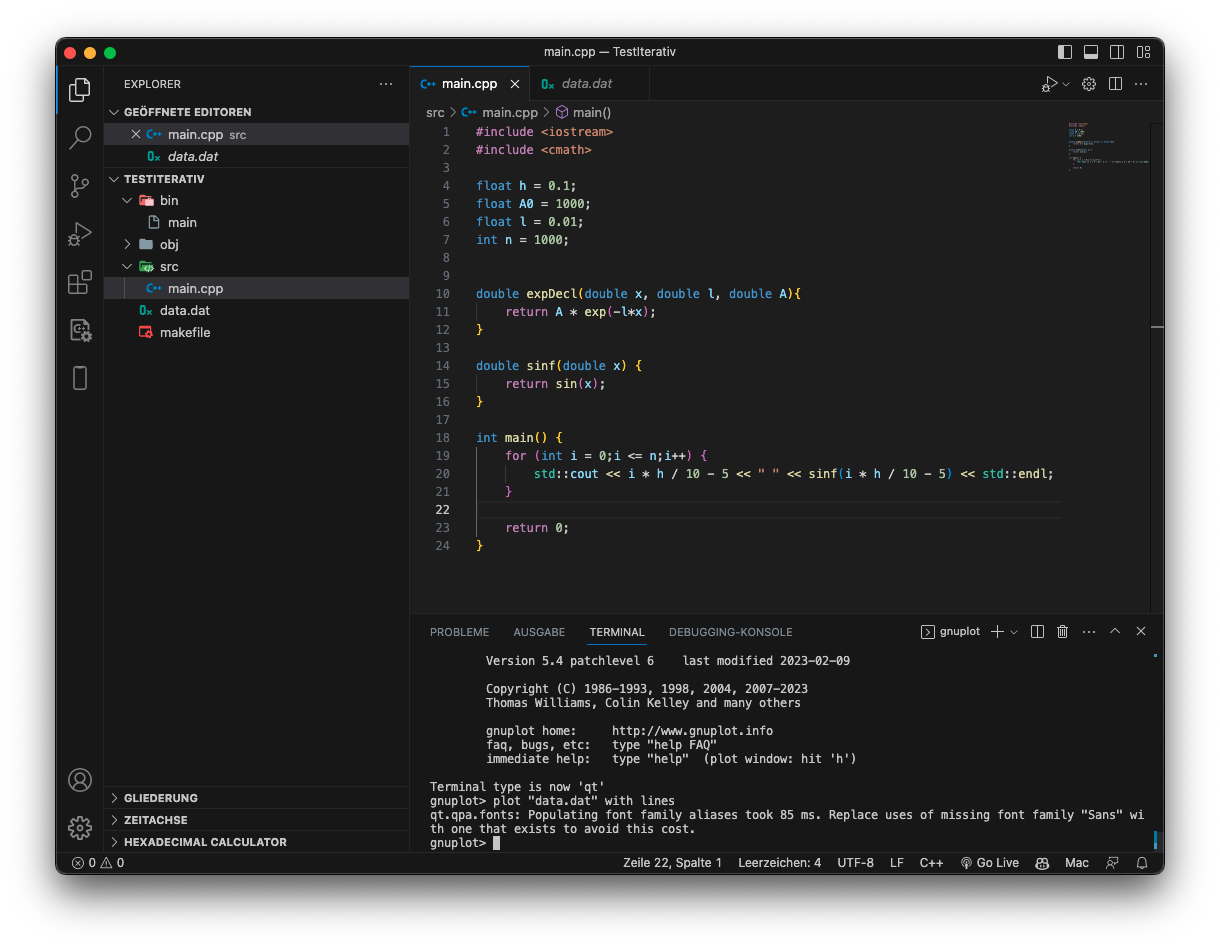
\includegraphics[width=\textwidth]{Bilder/Bildschirmfoto 2023-04-26 um 22.51.54.png}
            \caption{Code zum Plotten einer Sinusfunktion}
            \label{fig:gnuplotSinefunction}
        \end{figure}

         \begin{figure}[H]
            \centering
            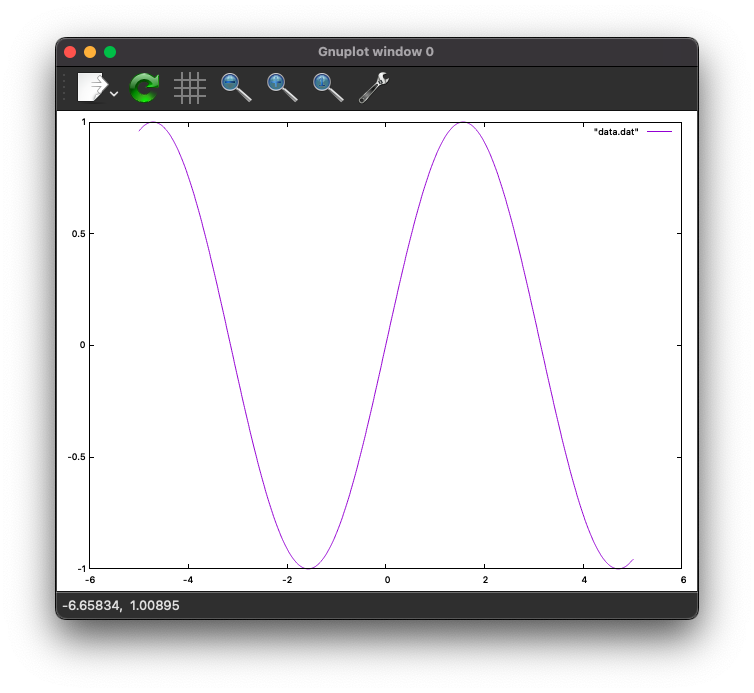
\includegraphics[width=0.6\textwidth]{Bilder/Bildschirmfoto 2023-04-26 um 22.51.30.png}
            \caption{Sinusfunktion im Intervall $x\in[-5,5]$ mit gnuplot geplottet}
            \label{fig:gnuplotSinefunction}
        \end{figure}
        
    \subaufgabe{}
        Der Befehl ls -l gibt das aktuelle Verzeichnis aus mit folgenden Format: [USERRIGHTS] - [LINSK TO FILESYSTEM?] - [USER] - [GROUP] - [SIZE] - [DATE OF CREATION] - [FILENAME].\\

        \noindent USERRIGHTS: ersten drei Ziffern stehen für Rechte des Eigentümers; die nächsten drei für die Ziffern der Gruppe; die letzten stehen für die Rechet aller weiteren Nutzer.

        \noindent Rechteverwaltung kann z.B. mit folgenden Commands verändert werden:
        \begin{itemize}
            \item chown [USER] [FILE] - USER kann die Datei FILE editieren/ hat Ownerrechte
            \item chgrp [USER] [FILE] - USER hat zugriff, die Datei zu lesen
            \item chmod [NUMBER] [FILE] - legt anhand eines Codes NUMBER (meistens vierstellig) fest, wer welche Zugriffsrechte auf FILE hat
        \end{itemize}

    \subaufgabe{}
        df gibt die Speicherverteilung/ die Belastung und verortung der Festplatten des PCs an. Für du siehe \textit{Aufgabe 2, (a)}.
        
\end{document}
    